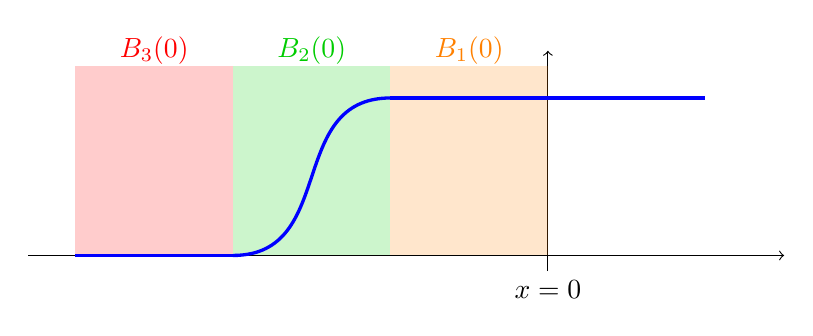
\begin{tikzpicture}[scale=2]
\draw[->] (-3.3, 0) -- (1.5,0);
\draw[->] (0, -0.1) node[anchor=north] {$x = 0$} -- (0, 1.3);
\fill[orange, opacity = 0.2] (0,0) rectangle (-1, 1.2);
\fill[green!80!black, opacity=0.2] (-1, 0) rectangle (-2, 1.2);
\fill[red, opacity=0.2] (-2, 0) rectangle (-3, 1.2);

\draw[blue, very thick] (-3, 0) -- (-2, 0) edge[out=360, in = 180, looseness = 1.2] (-1, 1);
\draw[blue, very thick] (-1, 1) -- (1,1);

\node[orange] at (-0.5, 1.3) {$\mathbb{B}_1(0)$};
\node[green!80!black] at (-1.5, 1.3) {$\mathbb{B}_2(0)$};
\node[red] at (-2.5, 1.3) {$\mathbb{B}_3(0)$};

\end{tikzpicture}
